\input{/Users/qinyulin/LaTex/Modules/ArticleClass/preamble}
\input{/Users/qinyulin/LaTex/Modules/ArticleClass/contents}
\input{/Users/qinyulin/LaTex/Modules/ArticleClass/mathequ}
\input{/Users/qinyulin/LaTex/Modules/ArticleClass/environments}
\input{/Users/qinyulin/LaTex/Modules/ArticleClass/tables}
\input{/Users/qinyulin/LaTex/Modules/ArticleClass/figures}
\input{/Users/qinyulin/LaTex/Modules/ArticleClass/float}
\input{/Users/qinyulin/LaTex/Modules/ArticleClass/colors}
\input{/Users/qinyulin/LaTex/Modules/ArticleClass/fancypage}
\setlength{\droptitle}{-2cm}
\pretitle{\begin{center}\LARGE\sffamily}
\title{固体理论阅读笔记}
\posttitle{\par\end{center}\vspace{-0.3cm}}
\preauthor{\large}
\DeclareRobustCommand{\authorthing}
{
\begin{center}
\begin{tabular}{c}%cc}
覃宇林\\
\end{tabular}
\end{center}
}
\author{\authorthing}
\postauthor{}
\predate{\begin{center}\large\scshape}
\date{2021年10月01日}
\postdate{\par\end{center}}

\begin{document}
%pagestyle{plain}
\frontpagestyle
\maketitle
\pagenumbering{Roman}
\tableofcontents\newpage
\pagenumbering{arabic}
\mainpagestyle
\setcounter{page}{1}

\section{周期性结构}
\subsection{Lie Groups and Their algebra}
对于一个李群,定义其在单位元处的切空间为其李代数:
\[g:=T_1G\]
关于李群有相关的映射及其诱导的切空间之间的映射,如图\ref{fig:basicmap} 所示。
\begin{figure}
\begin{center}
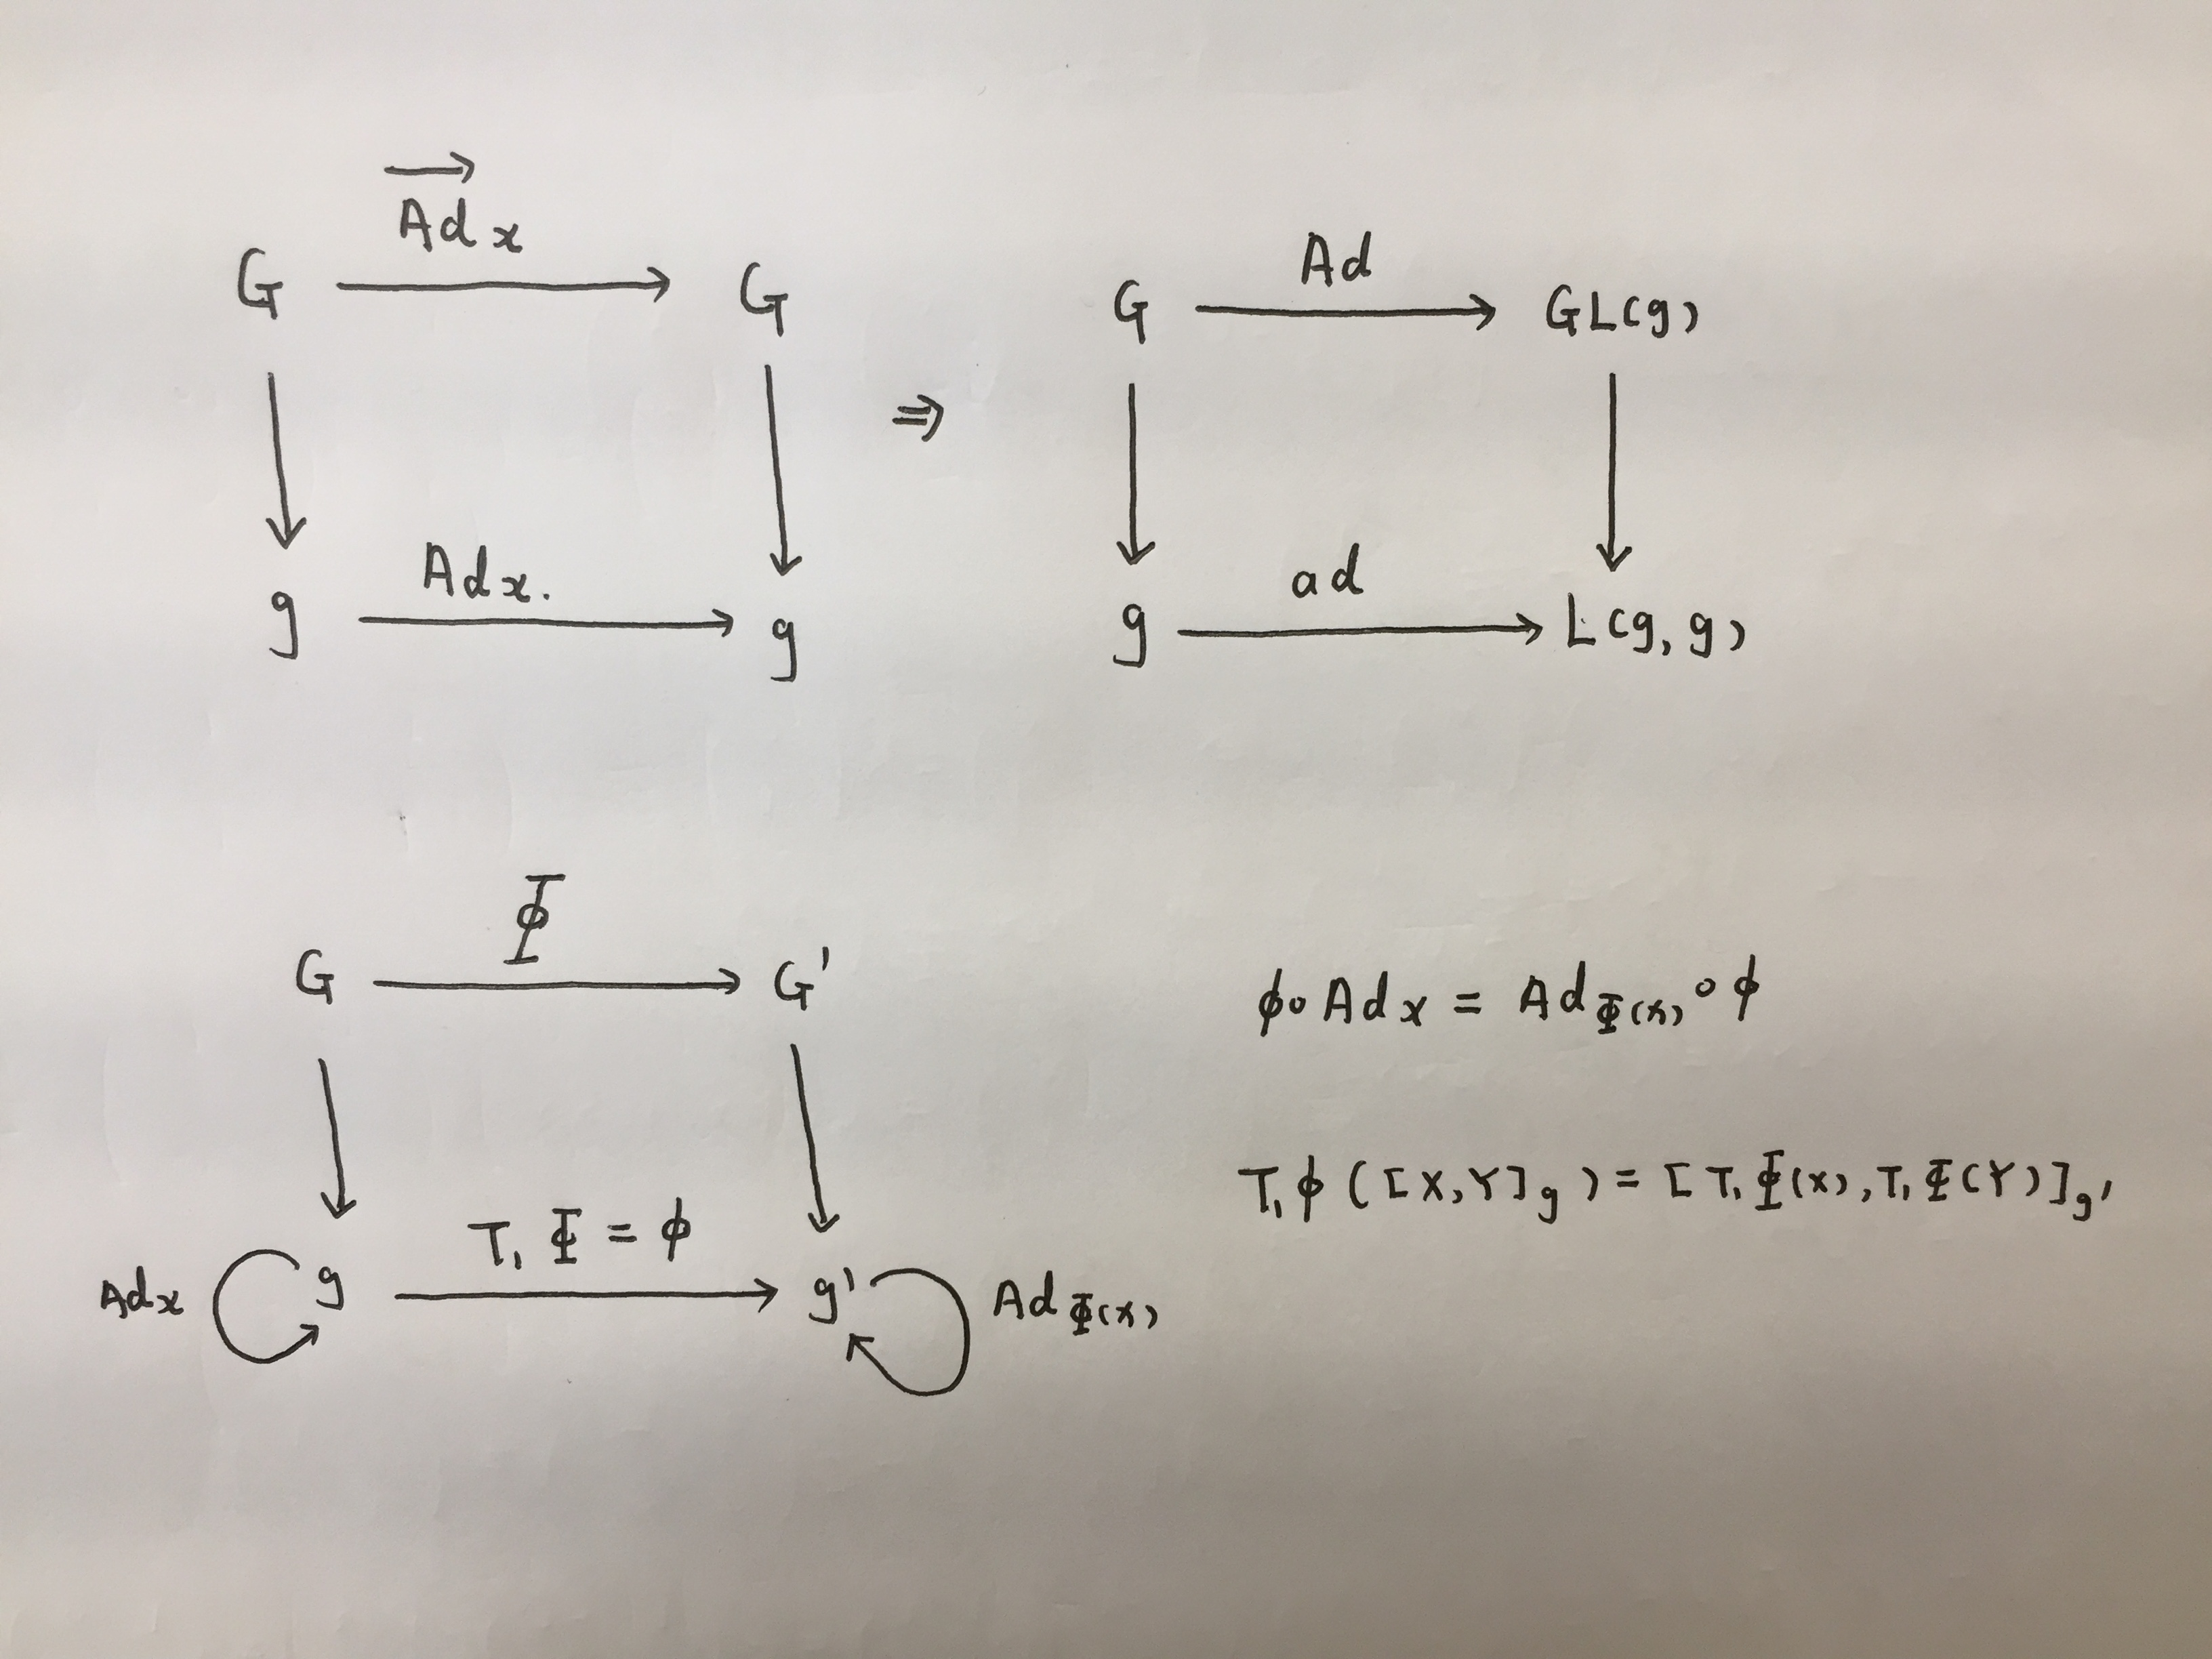
\includegraphics[height=8cm]{figures/Mappings.JPG}
\caption{李群之间的基本映射}
\label{fig:basicmap}
\end{center}
\end{figure}
其中我们有:
\[ad(X)(Y)=[X,Y]\]
李括号之间的基本性质:
\[[X,[Y,Z]]+[Y,[Z,X]]+[Z,[X,Y]]=0\]
常见的李群之正交群
\[O(n,R)=\{A\in L(R^n,R^n)|A^TA=I\}\]
它的李代数为:
\[o(n,R)=\{X\in L(R^n,R^n)|X^T+X=0\}\]
特殊正交群:
\[SO(n,R)=\{A\in O(n,R)|det(A)=1\}\]
它的李代数为:
\[so(n,R)=\{X\in L(R^n,R^n)|X^T+X=0 tr(X)=0\}\]
对于SO(3,R)中的元素,可以表示为:
\[R_x=I+\frac{sin|x|}{|x|}A_x+\frac{1-cos|x|}{|x|^2}A_x^2\]
其中x为$R^3$中的元素且:
\begin{equation}
A_x=\left(\begin{array}{ccc}
0&-x_3&x_2\\
x_3&0&-x_1\\
-x_2&x_1&0\\
\end{array}
\right)
\end{equation}

也就是说,这给出了从$R^3$到SO(3,R)中的元素的一个映射。\par
SO(3,R)中的共轭类为:
\[C_c=\{R_x|x\in R^3,|x|=c\}\]
且他的基本群为:
\[\pi_1(SO(3,R))=Z/2Z\]
Unitary Group:
\[U(n)=\{A\in L_C(C^n,C^n)|A^\dagger A=I\}\]
它的李代数为:
\[u(n)=\{A\in L_C(C^n,C^n)|A^\dagger+A=0\}\]
Special Unitary Group:
\[SU(n)=\{A\in U(n)|det(A)=1\}\]
它的李代数为:
\[su(n)=\{A\in u(n)|tr(A)=0\}\]
对于SU(2),我们有:
\[SU(2)=\{\left(\begin{array}{cc}a&b\\-\bar{b}&\bar{a}\\\end{array}\right)|a,b\in C,|a|^2+|b|^2=1\}\]
SU(2)的共轭类为:
\[C_c=\{A\in SU(2)|Re(a)=c\}\]
对于SU(2)的李代数,我们有:
\[su(2)=\{\left(\begin{array}{cc}i\alpha&\beta\\-\bar{\beta}&-i\alpha\\\end{array}\right)|\alpha\in R,\beta\in C\]
special linear group:
\[SL(n,R)=\{A\in L_R(R^n,R^n)|det(A)=1\}\]
它的李代数为:
\[sl(n,R)=\{A\in L_R(R^n,R^n)|tr(A)=0\}\]

\subsection{The Exponential Map}
左右平移算符:
\[R(x)y=yx\]
\[L(x)y=xy\]
对于左右平移算符,我们有:
\[R(x)L(y)=L(y)R(x)\]
\[L(xy)=L(x)L(y)\]
\[R(xy)=R(y)R(x)\]
对于流形上的左不变向量场v,我们定义为:
\[v_{L(x)y}=T_yL(x)v_y\]
对于流形上的右不变向量场v,我们定义为:
\[v_{R(x)y}=T_yR(x)v_y\]
流形上的左右不变向量场记为:
\[X^L,X^R\]
\begin{lemma}
Let $\Phi^t$ be a  the flow of a left or' right invariant vector field v on G.this is a $C^2$ mapping G$\rightarrow$ G satisfying:\par
\begin{center}
\begin{tabular}{cc}
$\Phi^t=R(\Phi^t(1))$&if v is left invariant\\
$\Phi^t=L(\Phi^t(1))$&if v is right invariant\\
\end{tabular}
\end{center}
\end{lemma}

\begin{theorem}
For Every $X\in g$ there is a unique homomorphism $h=h_X$:(R,+)$\rightarrow (G,\cdot)$ that is differentiable at t = 0 and satisfies $\frac{dh}{dt}(0)=X$ It is equal to the solution curve of both $X^L$ and of $X^R$ starting at the identity element of G. The flows of $X^L$ and of $X^R$ are globally defined for all $t \in R$
\end{theorem}
so with this theorem,we can define the exponetial map form g to G which yield as:
\[Exp(X)=h_X(1)\]
one can easily get that:
\[h_X(st)=h_{tX}(s)\]
then set s=1 one can get:
\[h_X(t)=exp(tX)\]

differential the above function with respect to t one can get:
\begin{center}
\begin{tabular}{cc}
$X=T_0(exp)(X)$&for any X$\in$ g\\
\end{tabular}
\end{center}
so $T_0(exp)$ is equal to the identity,and  the $C^1$ diffeomorphism from U onto V opposite to exp is called log.\par
\subsection{The exponetial map of vector space}
we can define :
\[e^A=\sum_k\frac{1}{k!}A^k\]
we set $A(t)=e^{tX}$ then:
\[\frac{dA(t)}{dt}=XA(t)=T_1R(A(t))(X)=X^R(A(t))\]
so A(t) is a flow of X which imply that:
\[exp(X)=A(1)=e^X\]
one can easily get the relation:
\[det(e^A)=e^{tr(A)}\]
\subsection{the tanget map of Exp}
\begin{lemma}
Let G, and H, be Lie groups, with Lie algebra equal to g, and h, respectively. Suppose that if> is a homomorphism: G $\rightarrow$ H that is differentiable at 1 $\in$ G. Then$\Phi(expX) = exp(T_1\Phi(X))$, for each $X\in g$.
\end{lemma}
\begin{theorem}
\[Ad(exp(X))=e^{ad(X)}\]
\[xe^Xx^{-1}=e^{(Ad_x)(X)}\]
\end{theorem}

\begin{theorem}
For any $X\in g$  the linear mapping $T_Xexp:g\rightarrow T_{exp(X)}G$ is given by:
\[T_Xexp=T_1R(exp(X))\circ \int_0^1e^{sadX}ds=T_1L(exp(X))\circ\int_0^1e^{-s adX}ds\]
\end{theorem}
which is illustrated in figure\ref{fig:TxExp1} and figure\ref{fig:TxExp2}\par
\begin{figure}
\begin{minipage}[t]{0.5\linewidth}
\centering
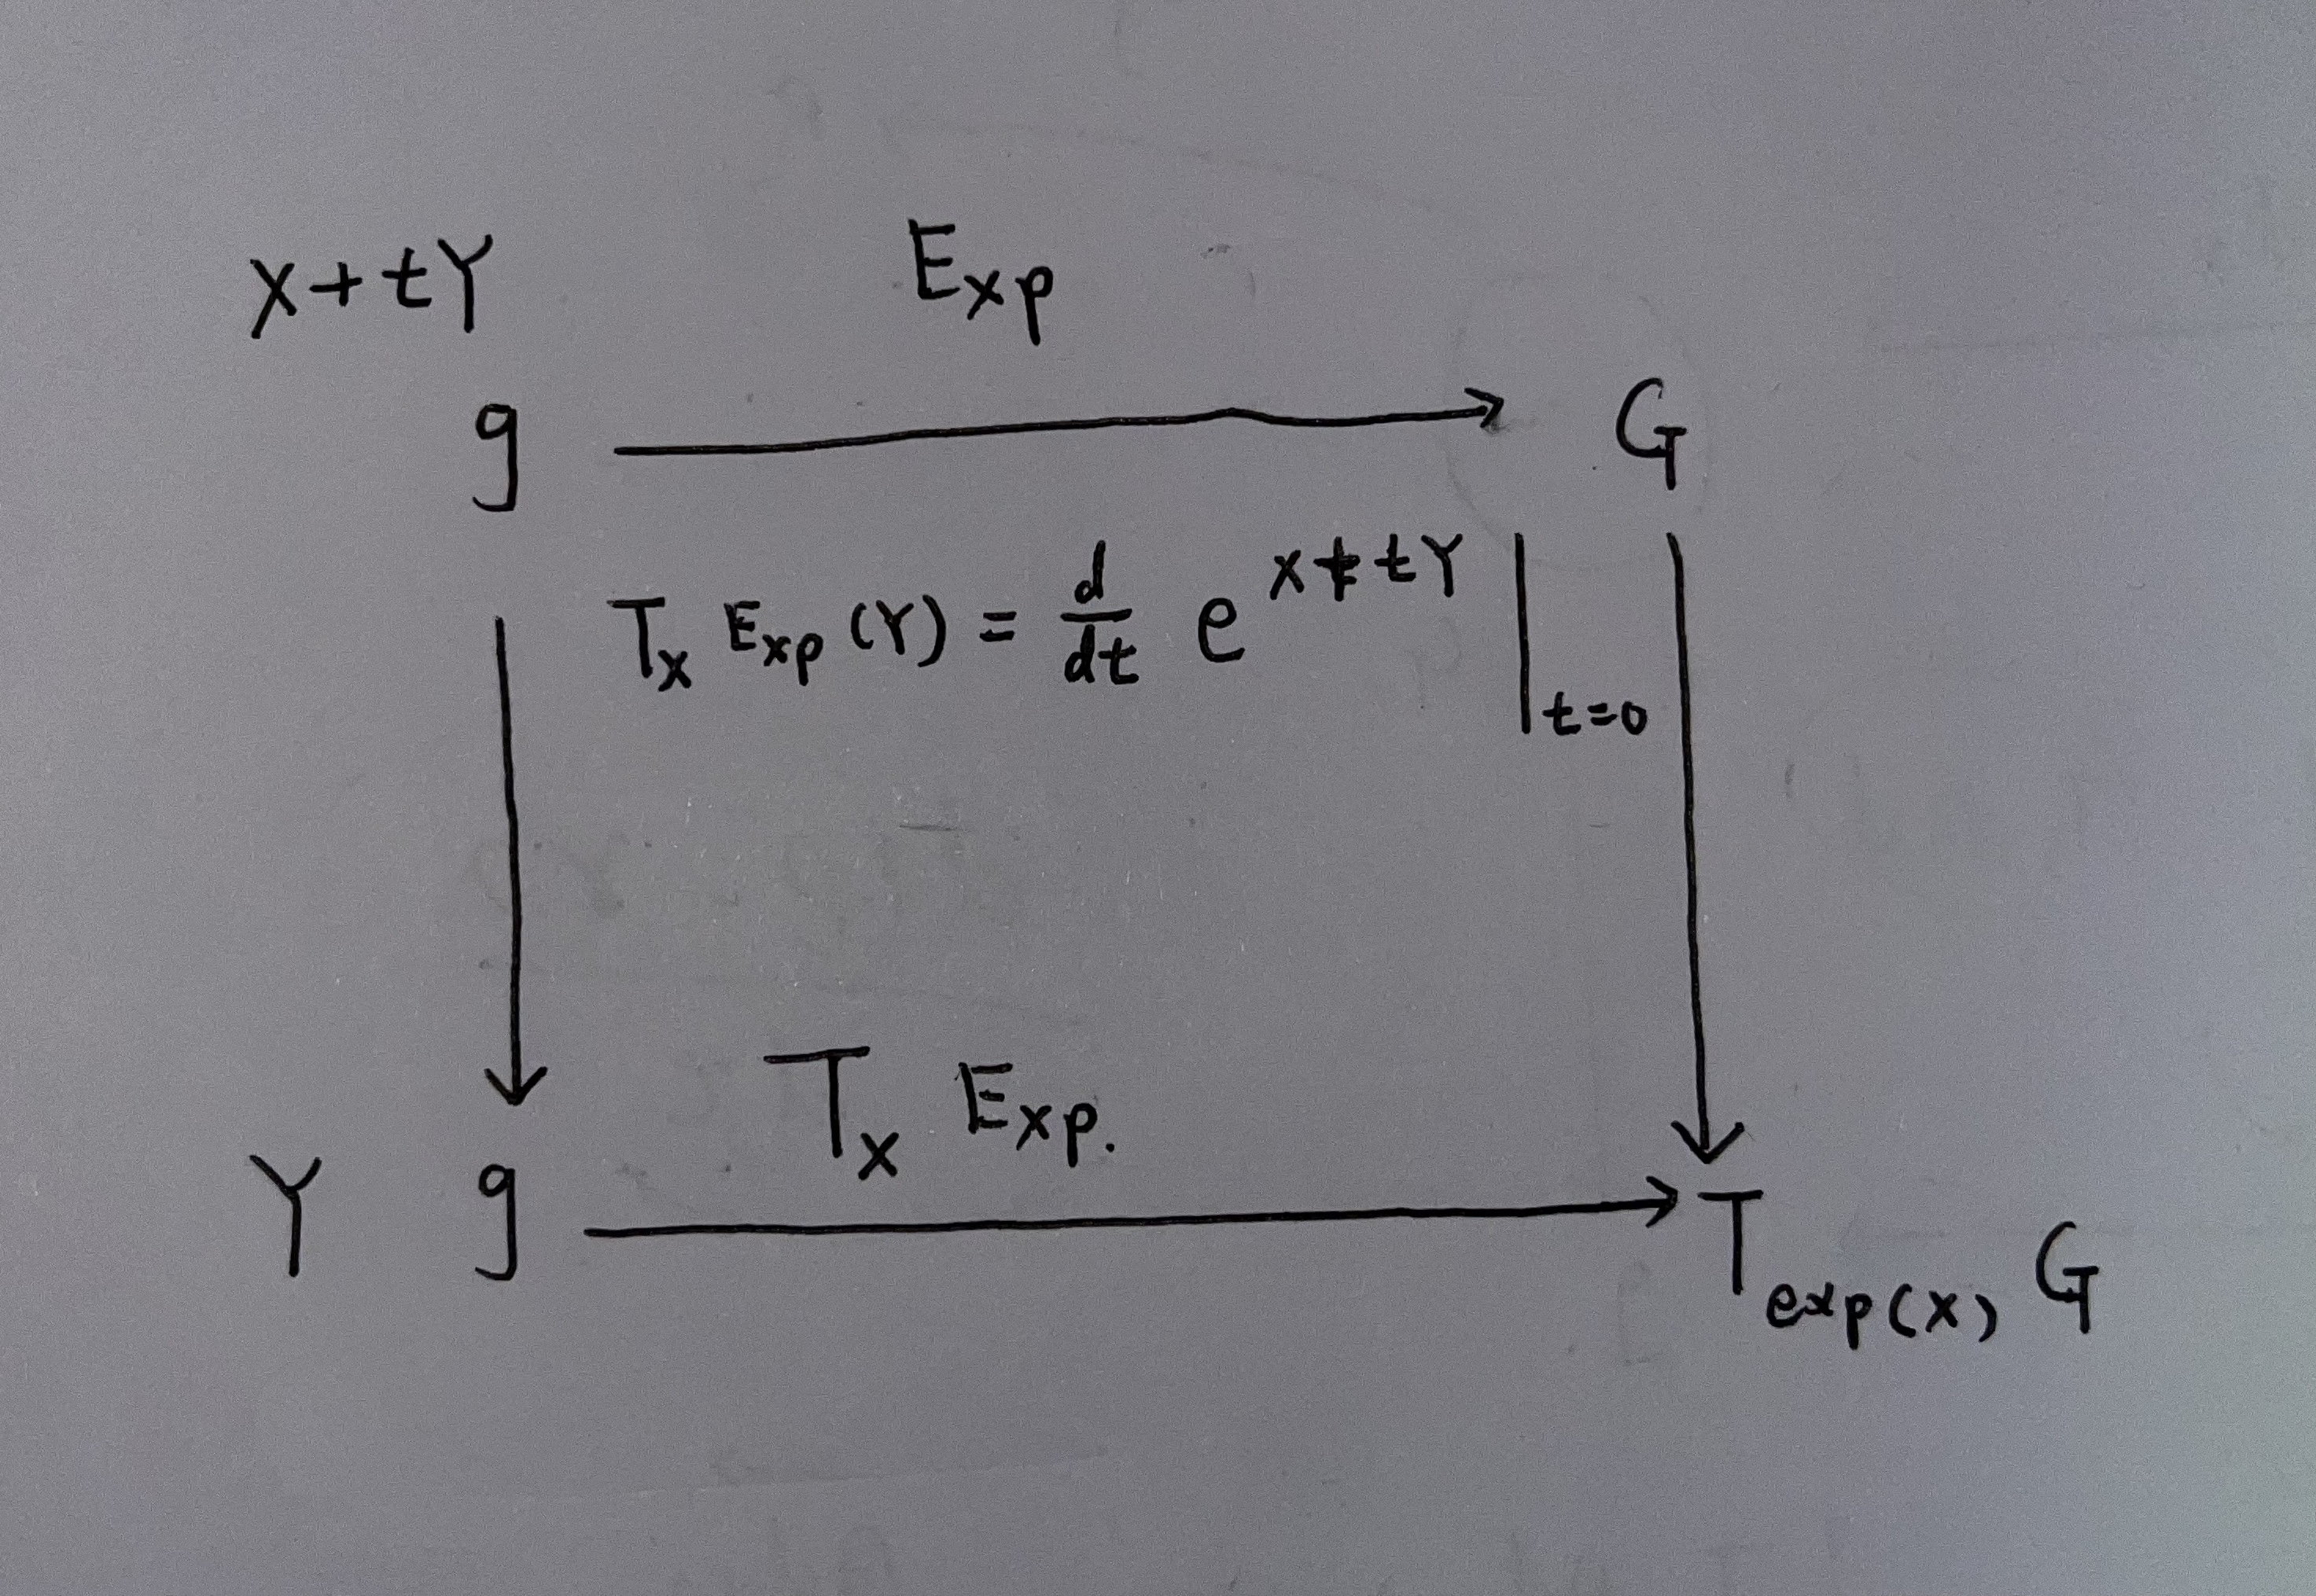
\includegraphics[width=\textwidth,height=6cm]{figures/TxExp1.jpg}
\caption{}
\label{fig:TxExp1}
\end{minipage}
\begin{minipage}[t]{0.5\linewidth}
\centering
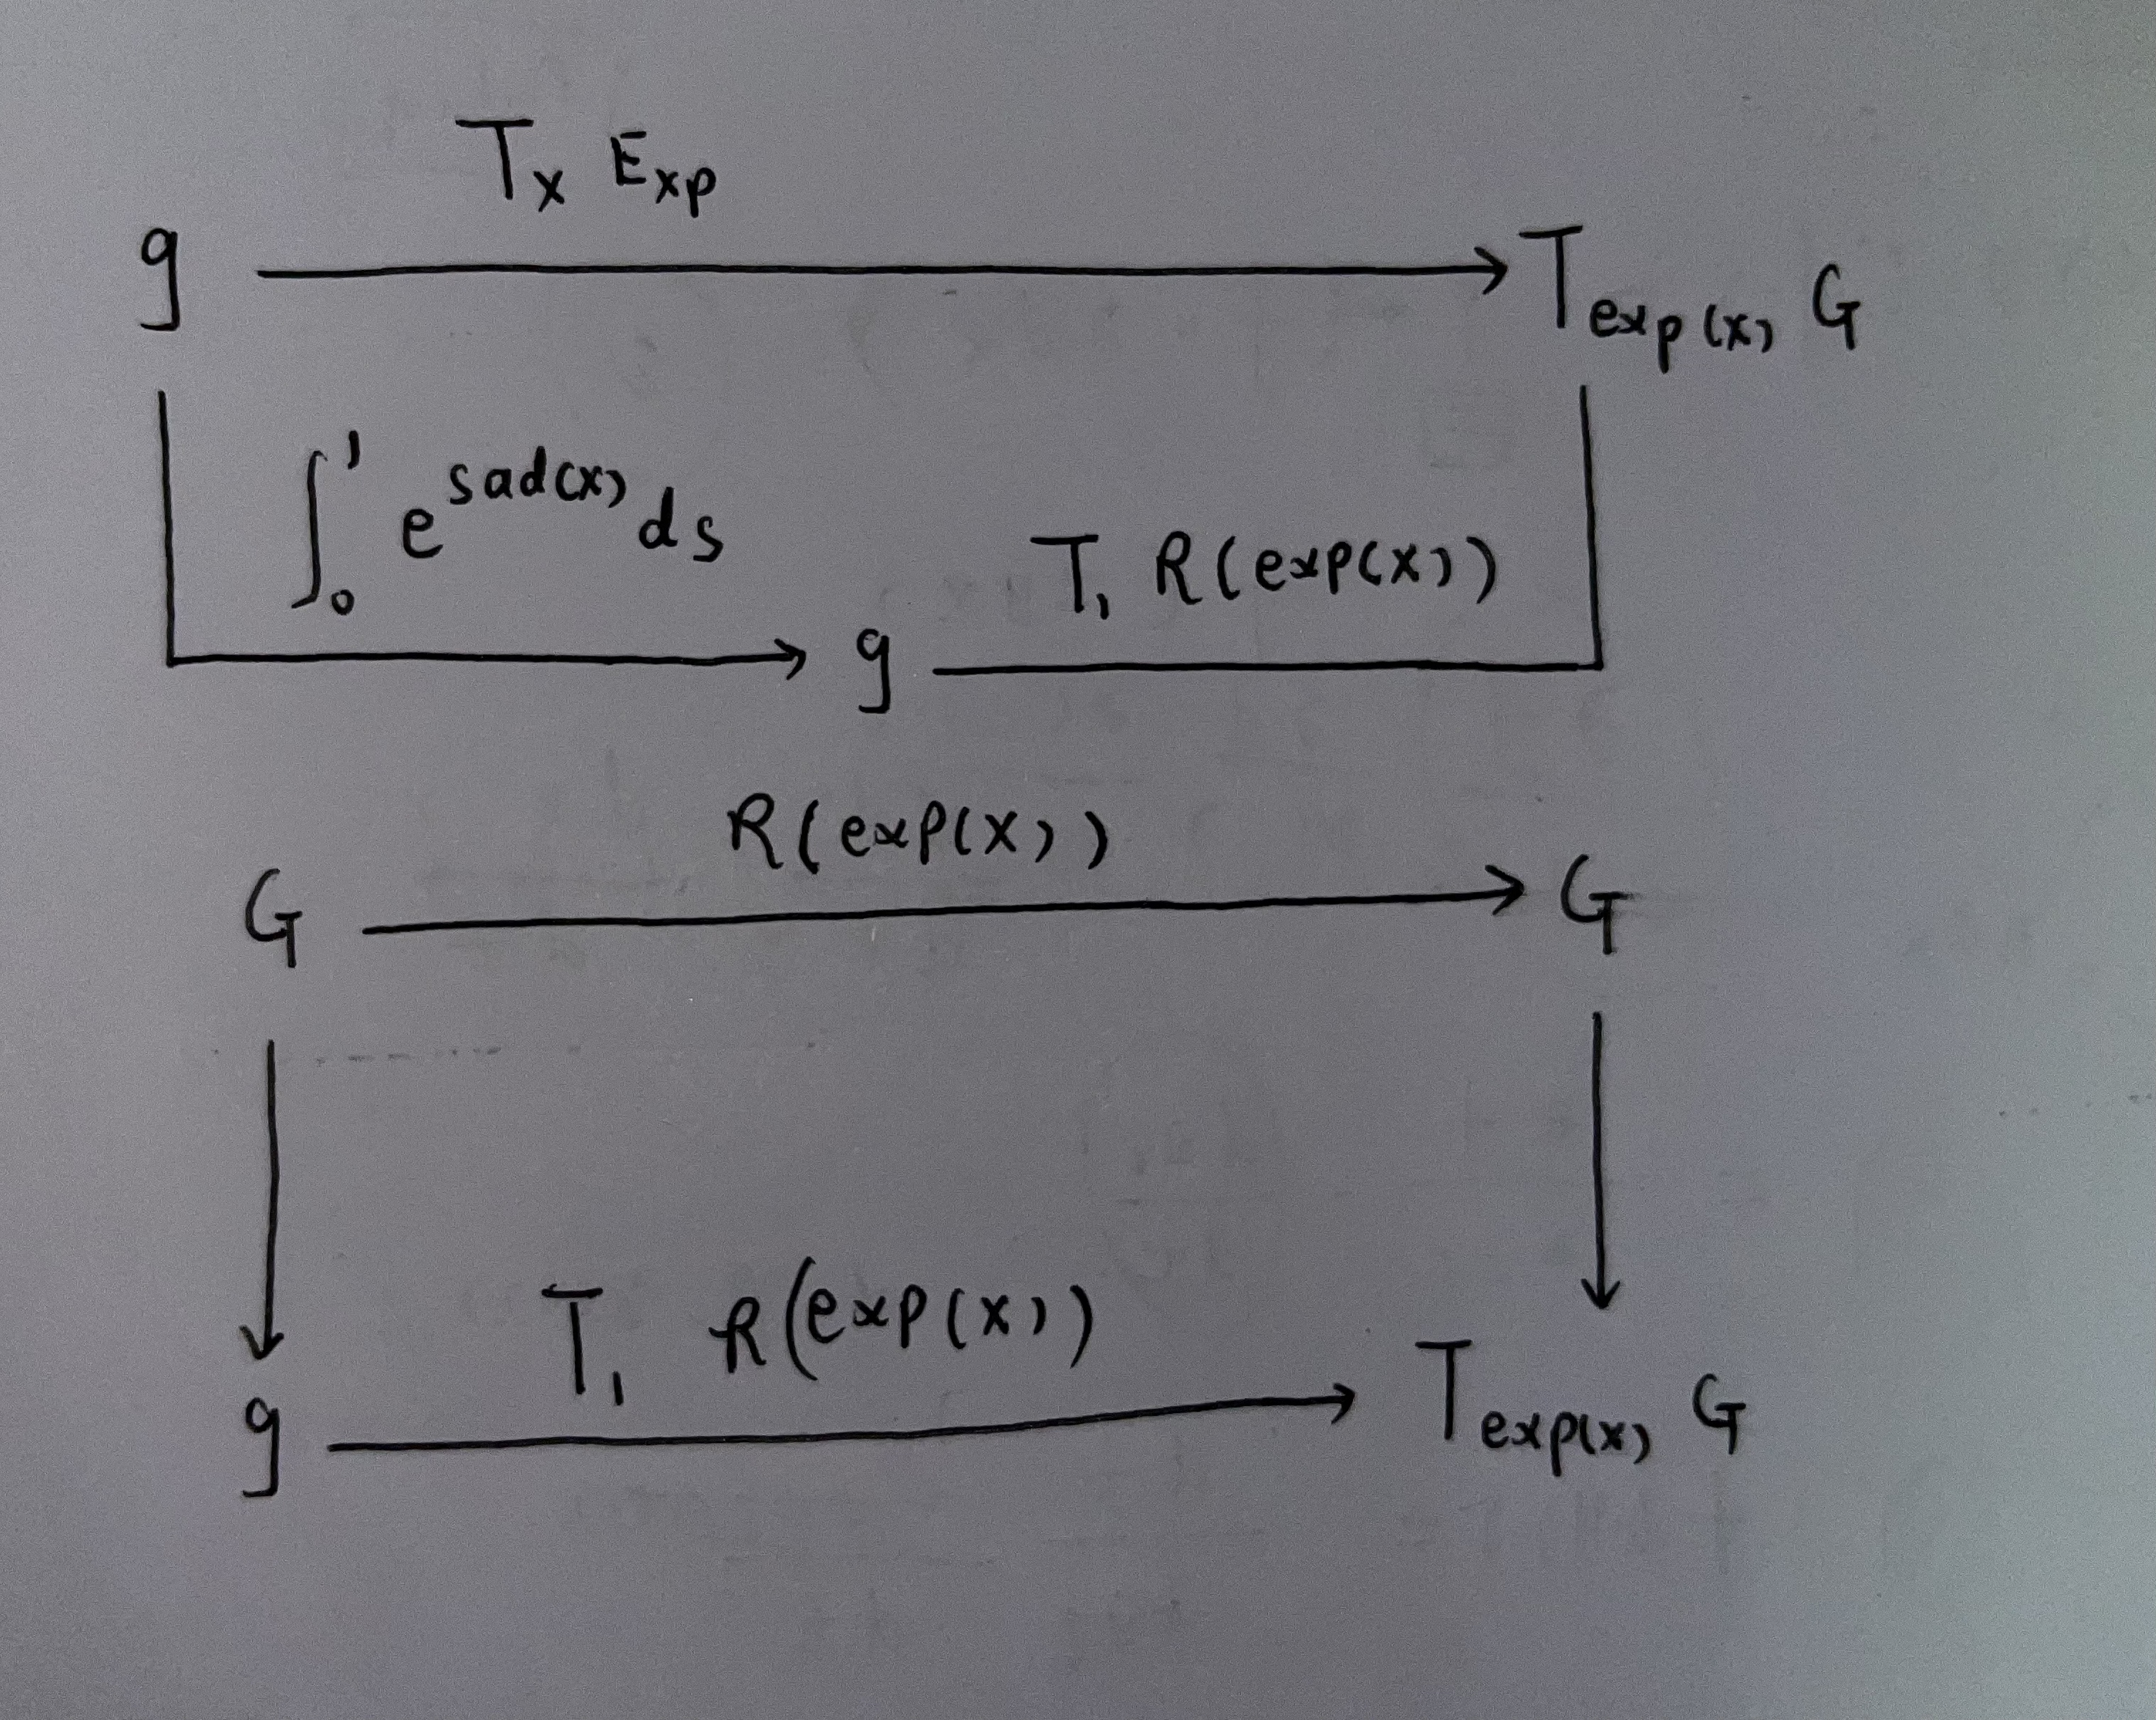
\includegraphics[width=\textwidth,height=6cm]{figures/TxExp2.jpg}
\caption{}
\label{fig:TxExp2}
\end{minipage}
\end{figure}

we can define a function of A as:
\[f(A):=\int_0^1e^{sA}ds=A^{-1}(e^A-I)\]
if A is invertible,then we have the corresponding definnition and if A is not invertible we define:
\[A^{-1}(e^A-I):=\int_0^1e^{sA}ds\]
\begin{lemma}
The singular points of the exponential mapping: $g \rightarrow G$, that is, the $X \in g$ such that $T_X$exp is not invertible, are precisely the $X \in g$ such that $ad X \in L(g, g)$ has an eigenvalue of the form $2\pi ik$, with $k \in Z \{O\}$
\end{lemma}
we can define the sets:
\[\Sigma_1:=\{X\in g| det(ad(X)-2\pi ik)=0\}\]
\subsection{The Product in Logarithmic Coordinates}
define a map from R to g which is:
\[t\in R \rightarrow (Z(t))\in g\]
that Z(t) satisfying the equation:
\[\frac{dZ(t)}{dt}=\frac{ad Z(t)}{e^{ad Z(t)}-I}(X), Z(0)=Y\]
set $g_e^2$ be the set of $(X,Y)\in(g,g_e)$ such the above solution is defined for all $t\in [0,1]$,make:
\[\mu(X,Y)=Z(1)\]
then we have the below theorem:
\begin{theorem}the set $g_e^2$ is an open neighborhood of (0, 0) in (g,g) and $\mu$ is a real-analytic mapping $g_e^2\rightarrow g$ .If g is the Lie algebra of a Lie group G, with exponential mapping exp then:
\[exp(X)exp(Y)=exp(\mu(X,Y))\]
\end{theorem}
 the mapping $\mu(X,Y)$ is called \textcolor{blue}{the product in logarithmic coordinates.}\par
pick up a open neigborhood of g in 0 $U_0$ then for the map:
\[V_0^x=L(x)exp(U_0)\]
\[k^x(y)=\ln(x^{-1}y)\]
we have the following theorem:
\begin{theorem}
The $k^x: V_0^x\rightarrow U_0$, for $x \in G$, form a real-analytic atlas for G, making G into a real-analytic Lie group $G_{an}$ , such that the identity in G is a $C^2$ diffeomorphism between G and $G_{an}$ . Furthermore, if g is a complex Lie algebra , then this atlas is complex-analytic. It makes G into a complex-analytic group if in addition $Ad_x$ is complex-linear: $g \rightarrow g$, for every $x \in G$.
\end{theorem}
\subsection{Dynkin's Formula}
\[\mu(X,Y)=X+Y+\sum_{k=1}^\infty\frac{(-1)^k}{k+1}\sum_{l_1\cdots l_k,m_1\cdots m_k\geq 0 ,l_i+m_i>0}\frac{1}{l_1+l_2+\cdots l_k}(\frac{(ad X)^{l_1}}{l_1!}\frac{(ad Y)^{m_1}}{m_1!}\cdots\frac{(ad X)^{l_k}}{l_k!}\frac{(ad Y)^{m_k}}{m_k!})(X)\]
so if $[X,[X,Y]]=0$ and $[Y,[X,Y]]=0$ then,we have:
\[\mu(X,Y)=X+Y+\frac{1}{2}[X,Y]\]
then we have:
\[e^Xe^Y=e^{X+Y+\frac{1}{2}[X,Y]}\rightarrow e^{X+Y}=e^Xe^Ye^{-\frac{1}{2}[X,Y]}\]



\section{声子}
\[\sum_{l'}\Phi_{\alpha\beta}(l-l')=0\]
利用哈密顿正则方程,可以得到晶体震动位移满足的方程为
\[M\frac{d^2}{dt^2}u_l^\alpha=-\sum_{l',\beta}\Phi_{\alpha\beta}(l-l')u_{l'}^\beta\]
利用布洛赫定理,晶体的震动应有:
\[u_l^\alpha=e^{ik\cdot R_l}u_0^\alpha\]
由此可以得到退耦合的方程。\par
定义一个动力矩阵:
\[D_{\alpha\beta}(k)=\frac{1}{M}\sum_{l}\Phi_{\alpha\beta}(l)e^{-ik\cdot R_l}\]
由正格矢量与倒格矢量之间的关系可知:
\[D_{\alpha\beta}(k)=D_{\alpha\beta}(k+K_n)\]
最后求解得到特解(只有k标记的模式):
\[u_l^\alpha\sim\frac{1}{\sqrt{N}}e_k^\alpha e^{i(k\cdot R_l-\omega(k) t)}\]
其中
\[De_k=\omega(k)^2 e_k\]
不同的k得到不同的特解,可以用此特解作为基函数展开晶格振动的一般解:
\[u_l^\alpha=\frac{1}{\sqrt{NM}}\sum_{k,\sigma}e^{\alpha}_{k\sigma}Q_{k\sigma}e^{ik\cdot R_l}\]
对于复式晶格,假设每个晶胞内有r个原子,其动力学矩阵为:
\begin{equation}
D_{\alpha\beta}\left(\begin{array}{c}k\\s,s'\\\end{array}\right)=\frac{1}{\sqrt{M_sM_{s'}}}\sum_{l}\Phi_{\alpha\beta}\left(\begin{array}{c}l\\s,s'\\\end{array}\right)e^{-ik\cdot R_l}
\end{equation}
相应的动力学矩阵的本征方程为:
\begin{equation}
\sum_{\beta,s'}D_{\alpha\beta}\left(\begin{array}{c}k\\s,s'\\\end{array}\right)e^\beta_k(s')=w^2e^\alpha_k(s)
\end{equation}

\subsection{格波特性}
由于$\omega(k)$是动力矩阵的本征值,而动力矩阵具有周期性,因此$\omega(k)$也具有周期性:
\[\omega(k)=\omega(k+K_n)\]
由于做了一个点群操作之后,动力学矩阵之间相差一个相似变换,本征值不变,因此$\omega(k)$具有晶体所属点阵的点群的全部对称性:
\[\omega(k)=\omega(\beta k)\]
由于$\Phi(x)$是实函数,因此动力学矩阵满足:
\[D(k)=D(-k)^*\]
因此得到其本征值之间的关系:
\[\omega^2(k)=\omega^2(-k)\rightarrow \omega(k)=\omega(-k)\]
对于$w(0)=0$的格波称为声学模,对于$w(0)\ne0$的格波称为光学模。
简单晶格中,对于k=0,由于有:
\[D(0)=0\]
因此全部为声学模。对于确定的$w_\sigma(k)$本征值,声学模在长波限下满足条件:
\[\frac{e_{\Gamma\sigma}^\alpha(s)}{\sqrt{M_s}}=\frac{e_{\Gamma\sigma}^\alpha(s')}{\sqrt{M_s'}}\]
因此说明元胞内的原子之间是同向运动,对于每一个k,有三个独立的声学模。相应的光学模在长波极限下满足(2个原子的复式晶格):
\[\sqrt{M_1}e_{\Gamma\sigma}^\alpha(1)=-\sqrt{M_2}e_{\Gamma\sigma}^\alpha(2)\]
因此光学模代表晶胞内原子的质心不动,原子相对于质心的运动,对于每个k,有3r-3个光学模。
\subsection{简正坐标}
不同的k得到不同的特解,可以用此特解作为基函数展开晶格振动的一般解:
\[u_l^\alpha=\frac{1}{\sqrt{NM}}\sum_{k,\sigma}e^{\alpha}_{k\sigma}Q_{k\sigma}e^{ik\cdot R_l}\]
其中$Q_{k\sigma}$为简正坐标,引入正则动量
\[P_{k\sigma}=\frac{\partial L}{\partial \dot{Q_{k\sigma}}}=\dot{Q}_{k\sigma}^*\]
最后哈密顿量可以写为:
\[H=\frac{1}{2}\sum_{k\sigma}\{P_{k\sigma}^*P_{k\sigma}+Q_{k\sigma}^*Q_{k\sigma}\}\]
作傅立叶逆变换表明$Q_{k\sigma},P_{k\sigma}$是系统的集体坐标与动量。\par
对这个系统进行量子化,由对每个格点的正则量子化条件:
\[[p_l^\alpha,u_{l'}^\beta]=-i\hbar\delta_{l,l'}\delta_{\alpha,\beta}\]
\[[p_l^\alpha,p_{l'}^\beta]=0,[u_l^\alpha,u_{l'}^\beta]=0\]
可以推导得出对于集体坐标的正则量子化条件:
\[[P_{k,\sigma},Q_{k',\sigma'}]=-i\hbar\delta_{k,k'}\delta_{\sigma,\sigma'}\]
\[[P_{k,\sigma},P_{k',\sigma'}]=0,[Q_{k,\sigma},Q_{k',\sigma'}]=0\]
由于之前的哈密顿量不是谐振子系统的形式,做正则变换:
\[a_{k\sigma}=\sqrt{\frac{\omega_\sigma(k)}{2\hbar}}(Q_{k\sigma}-\frac{P_{-k\sigma}}{i\omega_\sigma(k)})\]
\[a_{k\sigma}^\dagger=\sqrt{\frac{\omega_\sigma(k)}{2\hbar}}(Q_{-k\sigma}+\frac{P_{k\sigma}}{i\omega_\sigma(k)})\]
那么系统的哈密顿量为:
\[H=\sum_{k,\sigma}\hbar\omega_\sigma(k)(a_{k\sigma}^\dagger a_{k\sigma}+\frac{1}{2})=\sum_{k,\sigma}H_{k,\sigma}\]
代表3N种不同$(k,\sigma)$的无相互作用的声子系统,总能量:
\[E=\sum_{k,\sigma}(n_{k,\sigma}+\frac{1}{2})\hbar\omega_\sigma(k)\]
说明晶格振动的激发状态。可以用3N个数$\{n_{k,\sigma}\}$来描述\par
声子是格波激发的量子,称为集体震荡的元激发或准粒子。\par
\subsection{长波方法-声学模式}
这时模型可以过渡到连续介质情形,定义密度:
\[\rho=\frac{M}{\Omega}\]
系统动能:
\[T=\int d\tau \frac{1}{2}\rho\sum_\alpha \dot{u}^\alpha\dot{u}^\alpha\]
系统的势能:
\[\Delta\Phi=\int d\tau \frac{1}{2}\sum_{\alpha\beta,\mu,\nu}C_{\alpha\beta,\mu\nu}\frac{\partial u^\alpha}{r^\mu}\frac{\partial u^\beta}{r^\nu}\]
其中:
\[C_{\alpha\beta,\mu\nu}=-\frac{1}{2\Omega}\sum_l\Phi_{\alpha\beta}(l)(R_l)_\mu(R_l)_\nu\]
对这个系统进行量子化可以得到:
\[H=\sum_{k,\sigma}\hbar\omega_\sigma(k)(a_{k\sigma}^\dagger a_{k\sigma}+\frac{1}{2})=\sum_{k,\sigma}H_{k,\sigma}\]
\subsection{长波方法-光学模式}
对于元胞内有两个离子的离子晶体,定义相对运动矢量:
\[W=\rho^{\frac{1}{2}}(u_+-u_-)\]
其中的$\rho$为折合质量密度
那么系统的动能:
\[T=\frac{1}{2}\dot{W}\cdot\dot{W}\]
弹性势能:
\[\phi_1=\frac{1}{2}\gamma_{11}W\cdot W\]
极化部分的势能为:
\[\phi_2=-\int_0^EP\cdot dE\]
极化矢量由黄昆方程之一描述:
\[P=\gamma_{12}W+\gamma_{22}E\]
由此可以得到系统的哈密顿量为:
\[H=\frac{1}{2}\dot{W}\cdot\dot{W}+\frac{1}{2}\gamma_{11}W\cdot W-\gamma_{12}W\cdot E-\frac{1}{2}\gamma_{22}E\cdot E\]
由此可以得到光学模的运动方程(黄昆方程):
\[\frac{\partial^2 W}{\partial t^2}=-\gamma_{11}W+\gamma_{12}E\]
假设矢量的时间依赖关系为$e^{-iwt}$,那么可以得到介电函数与能量$\omega$的依赖关系:
\[\epsilon(\omega)=1+4\pi\{\gamma_{22}+\frac{\gamma_{12}^2}{\gamma_{11}-\omega^2}\}\]
由此可以得到几个重要的介电常数:
\[\epsilon_0=1+4\pi\{\gamma_{22}+\frac{\gamma_{12}^2}{\gamma_{11}-}\},\omega\le\omega_0\]
\[\epsilon_{infty}=1+4\pi\gamma_{22}\]
由此可以得到各个常数与介电函数的关系:
\begin{align}
\notag \gamma_{11}&=\omega_0^2\\
\notag \gamma_{12}&=(\frac{\epsilon_0-\epsilon_\infty}{4\pi})^{\frac{1}{2}}\omega_0\\
\gamma_{22}&=\frac{\epsilon_\infty-1}{4\pi}
\end{align}
将系统解为横波部分与纵波部分,那么横波部分的色散关系为:
\[\omega_T=\omega_0\]
纵波部分的色散关系为:
\[\omega_L^2=\gamma_{11}+\frac{4\pi\gamma_{12}^2}{1+4\pi\gamma_{22}}\]
由此可以得到著名的LST关系:
\[\omega_L^2=\frac{\epsilon_0}{\epsilon_\infty}\omega_T^2\]
而相应的介电函数可以表示为:
\[\epsilon(\omega)=\epsilon_\infty\frac{\omega_L^2-\omega^2}{\omega_T^2-\omega^2}\]
\subsection{极化激元}
光子-横光学模声子的耦合模式,其量子即为极化激元,是离子晶体中的元激发。\par
\subsection{态密度}
\[g(w)=\frac{1}{N}\sum_{k,\sigma}\delta(w-w_\sigma(k))\rightarrow \frac{\Omega}{(2\pi)^3)}\sum_\sigma\int_{\Omega^*}\delta(w-w_\sigma(k)d^3k\]
为了讨论其奇异行为,常常利用另外一种方式来表示态密度:
\[g(w)=\frac{\Omega}{(2\pi)^3)}\sum_\sigma\int_{S_\omega}\frac{dS_{\Omega\sigma}}{|\nabla_k\omega_\sigma(k)|}\]
当波包群速度$\nabla_k\omega_\sigma(k)$为零时,系统的态密度出现奇点,这个奇点称为范霍夫奇点。\par
\subsection{范霍夫奇点}



\end{document}